\subsection{}

\subsection{}
A hidden markov model can be defined as $\lambda = (\pi, m, e)$ where: $\pi$ are the initial probabilities, $m$ are the transition probabilities, and $e$ are the emission probabilities.
The goal of the Expectation Maximisation algorithm is to calculate a value of $\lambda$ that maximises $p(x|\lambda)$ for a given sequence of observed data $x$. As finding a global maximum is computationally intractable we use the Baum-Welch algorithm which gives us a local maximum. The Baum-Welch algorithm generates $\hat{\lambda}$ from $\lambda$ where $p(x|\hat{\lambda}) \geq p(x|\lambda)$. Iterating this process, where at each step we say $\lambda \gets \hat{\lambda}$, converges to a local optimum.

To calculate $\hat{\lambda}$ we can use some helper functions as described by L.R. Rabiner \cite{em}. We will use additional notation $N$ ass the number of hidden states, $O_t$ the observation at time (position) $t$ and $T$ as $|O|$.  The first helper function is $\alpha$, which is the forward algorithm.
\begin{gather*}
    \alpha_1(i) = \pi_i e_i(O_1)\\
    \alpha_{t+1}(i) = e_j(O_{t+1}) \cdot \sum_{i=1}^N\alpha_t(i)m_{ij}
\end{gather*}

The next $\beta$, which is the backward algorithm :
\begin{gather*}
    \beta_T(i)=1\\
    \beta_t(i)=\sum_{j=1}^N m_{ij} e_j(O_{t+1}) \beta_{t+1}(j)
\end{gather*}

Then $\gamma$ which is the probability of being in a state at a point in time, given we know which observations precede and succeed the current observation.
\begin{gather*}
    \gamma_t(i) = \frac{\alpha_t(i) \beta_t(i)}{\sum_{j=1}^N \alpha_t(j) \beta_t(j)}
\end{gather*}

And finally $\xi$, the probability of transitioning from state i to state j given we know all observations preceding i and succeeding j.
\begin{gather*}
    \xi_t(i, j) = \frac{\alpha_t(i) m_{ij} e_j(O_{t+1}) \beta_{t+1}(j)}{\sum_{i=1}^N \sum_{j=1}^N \alpha_t(i) m_{ij} e_j(O_{t+1}) \beta_{t+1}(j)}
\end{gather*}

Using these helper functions we can calculate $\hat{\lambda}=(\hat{\pi}, \hat{m}, \hat{e})$.
\begin{gather*}
    \hat{\pi}_i = \gamma_1(i)\biggbreak
    \hat{m}_{ij} = \frac{\sum_{t=1}^{T-1} \xi_t(i,j)}{\sum_{t=1}^{T-1} \gamma_t(i)}\biggbreak
    \hat{e}_i(k) \frac{\sum_{\forall t: O_t = k} \gamma_t(i)}{\sum_{t=1}^T \gamma_t(i)}
\end{gather*}


We can tackle verification of the algorithm using 2 methods: by testing helper function and by observing that the algorithm maximises $p(x|\lambda)$. I verified each helper function with unit tests that: verify base cases (if applicable); and verify against known mathematical identities. Following are a small sample of the 8 identities I test against. NOTE: a free index implies that the identity hold over domain of the index, in some cases I test across the whole domain, in others just a sample, depending on what is computationally feasible.

\begin{gather*}
    %\sum_i \alpha_t(i) = 1 \\ wrong
    \sum_{x \in \Sigma^*} \beta_0(i) = 1\\
    \sum_{i} \gamma_t{i} = 1\\
    %\sum_{i}\sum_{j} \xi_t(i, j)=1\\
    \sum_{j} \xi_t(i,j) = \gamma_t(i)\\
    %\sum_i \hat{\pi}_i = 1\\
    \sum_j \hat{m}_ij = 1\\
    %\sum_k \hat{e}_i = 1 \\
\end{gather*}


To validate that the algorithm maximises $p(x|\lambda)$ we can plot $p(x|\lambda)$ against the iteration. Figure \ref{fig:em} shows 2 experiments that both use a fixed $x$ with 5 random initial $\lambda$. We see in Figure \ref{fig:em} that in all 10 runs $p(x|\lambda)$ converges at various local maxima. Experiments using different $x$ and $\lambda$ yield similar results, as you would expect. This provides strong evidence that the algorithm is valid.

\begin{figure}[h!]
    \begin{center}
    \begin{subfigure}{.5\textwidth}
        \begin{center}
    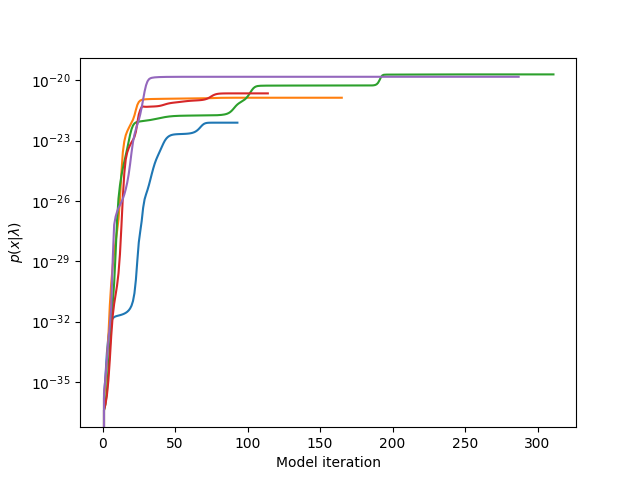
\includegraphics[width=.95\textwidth]{EM2.png}
    \caption{}
    \label{fig:em1}
    \end{center}
    \end{subfigure}%
    \begin{subfigure}{.5\textwidth}
        \begin{center}
        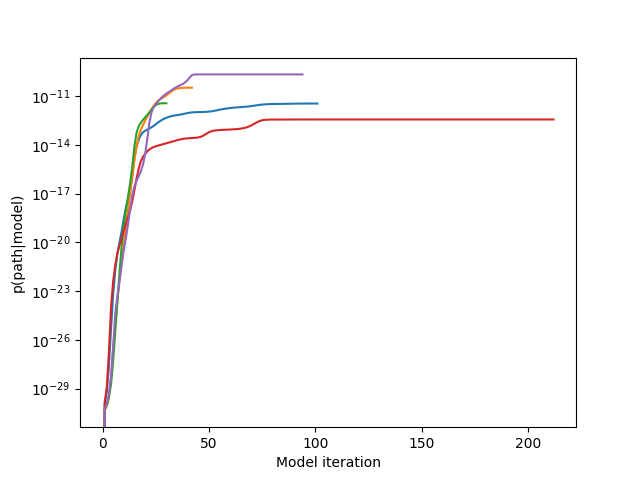
\includegraphics[width=.95\textwidth]{EM.png}
        \caption{}
        \label{fig:em2}
    \end{center}
        \end{subfigure}%
        \caption{Convergence of $p(x|\lambda)$ to local maxima for 2 values of $x$ each using 5 randomly initialised $\lambda$.}
    \label{fig:em}
    \end{center}
    \end{figure}